\section{Lead assessment and the next discriminating work}\label{sec:assessment}

\subsection{A concrete progress ledger}

The table below collects examples that answer ``what improved?'' without
collapsing unlike tasks into a single progress score. Ratios are
candidate/incumbent unless explicitly stated otherwise. A value below one
means less of the stated cost, not necessarily a faster complete ECDLP.
No cumulative factor is obtained by multiplying rows with different
inputs, baselines or boundaries.

\begin{longtable}{@{}p{3.7cm}p{3.1cm}p{3.5cm}p{3.1cm}@{}}\toprule
Concrete change & Recorded progress & Boundary and evidence & Remaining limit \\\midrule\endhead
Production free relations & 0.960 [0.946,0.976]; 360 verified runs &
Tuned complete counted IC comparison; engineering. \src{ROUND2} &
Small gain; not a sub-rho result \\
N83 smaller compact base & 2.645 s saved [2.085,3.205] & Five-point
cold-process holdout; engineering. \src{N83} & Two leading candidates
not significantly separated \\
Weighted D4 solver & About 18 times less than previous invariant form &
Decomposition constant, several primes, root checks; engineering.
\src{D4} & No complete-method $S$ in that study \\
D4 first-dependency stop & 0.979 [0.973,0.986] & Complete counted
comparison on 27 held-out curves. \src{ROUND2} & Extension-field toy regime \\
Genus-three matrix route & 0.653 [0.647,0.660] at $2^{20}$ & Complete
counted solve; 474 logs verified. \src{ROUND2} & Phase exponents and
source-to-Jacobian comparison remain distinct \\
F4 large matrix on RTX 5090 & 425.8 s to 5.70 s & Same task, ranks,
refutations and pinned variables. \src{F4-GPU} & Stage only; inherited
CPU wins another oracle boundary \\
H100 tiled update & 1.11--1.49 times faster & Historical device-stage
measurement; engineering. \src{F4-PANEL} & Upload and full-query costs remain \\
Inherited F4 & 198.6--222.1 times less matrix work & Identical-tree
stage comparison. \src{GB} & Not a uniform general-CAS speed claim \\
Factor-base degree predictor & MAE 0.06; 0.08 leaving out fields &
Empirical rule on 656 bases. \src{HEUR} & Not a proved scaling law \\
Symbolic twist-bit rule & 5,811 certified cases, zero counterexamples &
Finite certificate-backed observation. \src{ML-TWIST} & Global theorem
and independent semantic review are separate \\
Graph-wide instrument & 2,935 audited vertices, 46,960 attempts &
Actual checkpoint; manifest freshly checked. \src{VOL-ARCHIVE} &
11.8\% of declared smaller graph population \\
Native-toolkit reproducibility & 17 configured tests covered & Fresh
Release build, 15 initial passes plus two repaired-environment passes &
Core native tests, not every historical experiment \\\bottomrule
\end{longtable}

\begin{figure}[htbp]
\centering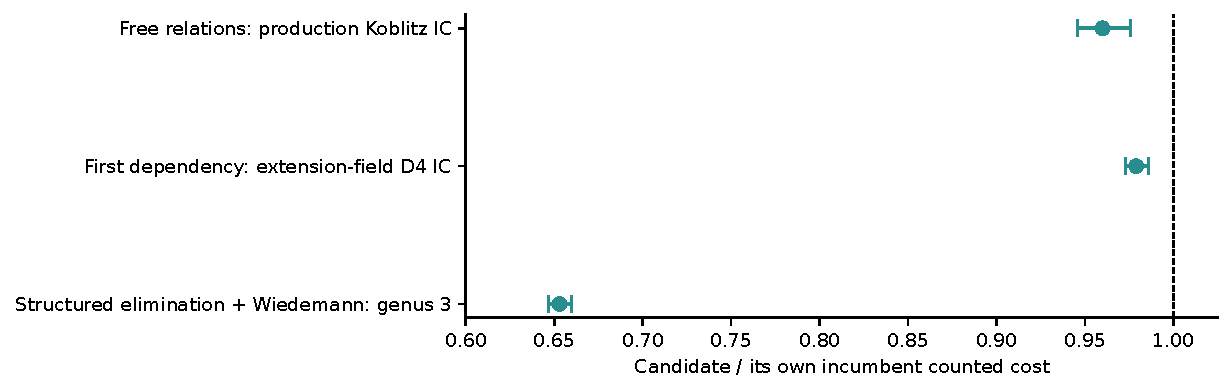
\includegraphics[width=\linewidth]{figures/incumbent-improvements.pdf}
\caption{Selected recorded candidate/incumbent comparisons. Each row
keeps its own task and baseline: the chart is a compact ledger, not a
ranking of methods or a cumulative speedup. Intervals are those reported
by the underlying studies. Sources: \src{ROUND2}.}
\end{figure}

These examples support four concrete conclusions. The programme has
built working instruments rather than only speculative notes. It has
made verified improvements over its own IC incumbents. It has developed
stronger controls that reverse some attractive interpretations. And it
still has a measured gap between its complete IC methods and the
strongest matched generic reference in the principal cold campaign.

\subsection{The ten open leads, without blanket closure}

The public ten-lead register preserves nineteen advisory records. Every
lead remains open in that register and no official hypothesis status is
changed by this paper. The observations below are what the register
reports; its private supporting packets were not freshly replayed here.
The proposed next steps are discriminating tests, not scheduled runs or
completed experiments.\src{TEN}

\begin{longtable}{@{}p{3.1cm}p{5.5cm}p{4.8cm}@{}}\toprule
Lead & What the record supports & Next discriminating obligation \\\midrule\endhead
1. Higher-arity refutation & A full-width timeout and memory error were
followed by compact row and kernel methods deriving one at degree four
on a specific negative system. Other degree-three closures do not refute
their named fixtures. & Freeze new negative and satisfiable controls;
compare full row spaces, proof sizes and complete costs. Do not infer a
minimum refutation degree from one closure. \\
2. Frobenius-equivariant F4 & The register's ordinary F4 fixture is
checked, but its complete character-block solver is not implemented.
Separate G2 passes elsewhere do not discharge that construction. &
Build one reconstructible character-block elimination stage over the
declared splitting field and verify the entire row space against F4. \\
3. Prime five-sum common factor & Six endpoint/evaluation arms agree on
the frozen queries; cached construction reduces counted calls in the
reported panel. The producer still enumerates $B^3$ endpoint occurrences. &
Seek an explicit construction avoiding that enumeration; test larger
primes with cold and warm setup charged. Tiny-field saturation is not
a scaling argument. \\
4. Reachable weak curves through covers & Eight declared rational
two-isogeny components over $\F_{7^6}$ are exhausted with no hit for one
norm-one branch-ratio criterion. A twist-commutation identity is scoped
to its stated transition. & Implement a concrete new transition,
independently verify its map and subgroup action, then search with
smoothness and field-of-definition gates. \\
5. Small-norm endomorphism closures & Two matched-advice methods recover
zero targets in 32 held-out attempts within 512 online steps; advice
logs are checked in the source record. & Require a structural coverage
prediction before enlarging the bank; compare norm and walk banks with
matched memory and charged setup. \\
6. Higher-arity torsion symmetry & The subgroup-only domain is not
stable under nonzero two-torsion translation at odd $r$. Suitable ambient
domains can be stable. & Construct a $T$-closed mixed-domain base and
quotient equations; compare to the same unquotiented domain and verify
every lifted solution. \\
7. Degree-131 higher-genus destination & The declared census produces
22 smooth models and five Weil classes. Finite order checks obstruct
particular homomorphisms for source primes above 263. & Produce an
explicit nonzero source/destination map with the required subgroup before
another candidate census; other targets remain open. \\
8. GPU F4 route & Seventy-six matrix/thread configurations pass host
device-source emulation and row-space replay in the register. Actual
GPU evidence elsewhere belongs to different tasks. & Run this frozen
panel on a device, then a complete-query paired comparison including
transfers, setup and replay. \\
9. Degree-83 relation control & Rank 600 and eight target logs in a
53-bit subgroup are reported using 32 imported and 568 new rows. &
Rebuild an entire smaller rank instance from zero and charge relation,
rank and target costs against rho. Imported work is not free. \\
10. XOR/PB curve-lift filtering & The register preserves filtered
resolutions and thirteen target precheck rejections, separately
attributed; satisfying an encoding alone is insufficient. & Freeze a
matched target panel, randomise arm order, price filter construction,
verify point lifting, and repeat under qualified isolation. \\\bottomrule
\end{longtable}

A timeout leaves an implementation or resource question; a finite
enumeration excludes its declared finite domain; a group-order argument
excludes its stated map class. Reopening a scoped obstruction requires a
changed load-bearing assumption or a challenge to the proof, rather than
merely a new name for the same construction. Conversely, no one of
these outcomes closes an entire mathematical direction.

\subsection{Priorities justified by the evidence}

\paragraph{First: complete the accounting and integrity bridges.}
Resolve the legacy S4 defect-impact audit, maintain root-call and native
counter emission on every arm, and co-measure the exact wide
equal-bytes preprocessing control. These actions determine what existing
figures mean; they do not require promising a new exponent. The audit
must retain environment drift and legacy-reproduction failures rather
than assigning every difference to the repaired expression.
\src{PR2412}\src{WIDE}

\paragraph{Second: answer one genuinely discriminating degree question.}
The $m=4,\ell=6$ closure cell separates the two surviving toy
explanations. The PKM $m=3,N=21$ trace now shows why a somewhat larger
host alone is not automatically enough: the next dense object has a
derived 317-GB payload before overhead. A new sparse or blocked engine
must reproduce the same closure and controls; a larger host must retain
the same protocol and an explicit stop. Neither approach should change
the mathematical question simply to make a run finish.\src{DREG}\src{PR2160}

\paragraph{Third: integrate component improvements into complete IC.}
The factor-base product-profile rule, root harvesting, calibrated sparse
linear algebra, weighted invariant systems and selected GPU stages are
concrete candidates. Each needs a held-out comparison to the current
incumbent with every phase charged. A positive component result can be
reported immediately at that boundary; it becomes a method improvement
only after the complete comparison moves.

\paragraph{Fourth: pursue transfers through explicit maps.}
Graph coverage can expand, but the next decisive transfer experiment
should name a source subgroup, a verified route, a destination solver
and a source-to-answer comparator. A larger collection of low-genus
objects without a subgroup bridge is not a substitute. For a graph
effect, hold subgroup size, target construction and base convention
fixed or model them explicitly, and keep sampled coverage separate
from complete populations.

\paragraph{Fifth: make learning choose a paid decision.}
The positive symbolic results justify using ML as a candidate generator.
The blind hardness nulls argue for targeting a specific useful decision
rather than another unadjusted global score. A base or solver policy
should outperform a simple constant policy on held-out classes after
feature extraction, inference and failures are charged. Any learned
rule that becomes a mathematical claim needs an exact statement and
independent verification beyond predictive accuracy.

\paragraph{Sixth: strengthen the proof-to-report map.}
Build the concrete-to-abstract bridges listed by CryptoLean, inspect
transitive axioms, and independently check that each report theorem has
the same quantifiers, exceptional cases, fields and subgroup hypotheses
as its formal declaration. Formalising a smaller algebraic identity is
valuable; it must remain labelled as that identity if the full claimed
cryptographic implication is still open.\src{LEAN}

\subsection{What the programme has learned}

The central lesson is operationally precise: the bottleneck can move,
and the comparison must move with it. Eliminating expensive polynomial
machinery can expose relation yield; faster relations can expose rank
generation; faster rank generation can expose setup or target work;
and a better generic reference can erase an apparent method advantage.
The programme's strongest progress is the combination of implemented
improvements and instruments able to show that a preferred explanation
was wrong.

The result is a broad collection of verified toy mechanisms, useful
algebraic and systems components, measured incumbent improvements,
structural conjectures with finite evidence, and named open obligations.
It is a foundation for continued ECDLP research whose next successes
can be measured against explicit baselines. It is not yet an
established general ECDLP exponent advance.
